\begin{center}

\includegraphics[width=0.5\textwidth]{content/3/chapter5/images/2.png}\\
Cippi开启了流水作业
\end{center}

由于C++20中的范围库,使用标准模板库(STL)变得更加好用和强大。范围库使用惰性算法,可以直接在容器上工作,并且可以很容易地组合。简而言之:范围库的简单和强大基于其思想。

深入讨论细节之前,先来看一个范围库的例子:

\hspace*{\fill} \\ %插入空行
\noindent
\textbf{结合transform和filter函数}
\begin{lstlisting}[style=styleCXX]
// rangesFilterTransform.cpp
#include <iostream>
#include <ranges>
#include <vector>
int main() {
	std::vector<int> numbers = {1, 2, 3, 4, 5, 6};
	auto results = numbers | std::views::filter([](int n){ return n % 2 == 0; })
						   | std::views::transform([](int n){ return n * 2; });
	for (auto v: results) std::cout << v << " "; // 4 8 12
}
\end{lstlisting}

必须从左到右读这个表达式。管道符号代表函数组合:首先,所有偶数都可以通过(std::views::filter([](int n)\{return n \% 2 == 0;\}))。之后,每个剩余的数字会映射到双倍功能上(std::views::transform([](int n)\{return n * 2;\}))。这个示例展示了范围库的两个新特性:可以将函数组合,应用于单个容器。

接下来,来了解一下范围(range)和视图(view)。

\subsubsubsection{5.1.1\hspace{0.2cm}范围和视图}

在关于概念的章节中,我已经介绍了范围和视图,这里简单复习一下。

\begin{itemize}
\item 
范围(range)是一组可以迭代的项,提供了一个开始迭代器和一个结束哨兵,STL容器也属于范围。
\end{itemize}

视图是在范围上执行的一些操作。视图不拥有数据,其复制、移动或赋值的时间复杂度恒定。

\hspace*{\fill} \\ %插入空行
\noindent
\textbf{在范围上操作的视图}
\begin{lstlisting}[style=styleCXX]
std::vector<int> numbers = {1, 2, 3, 4, 5, 6};
auto results = numbers | std::views::filter([](int n){ return n % 2 == 0; })
                       | std::views::transform([](int n){ return n * 2; });
\end{lstlisting}

这个代码片段中,numbers是范围,std::views::filter和std::views::transform是视图。

C++20的视图有助于函数式编程。视图可以组合,并且是惰性的。我已经介绍了两种视图,但C++20提供了更多的视图。

\begin{table}[H]
\centering
\begin{tabular}{ll}
视图                                                                                         & 描述                                              \\ \hline
\begin{tabular}[c]{@{}l@{}}std::views::all\_t\\ std::views::all\end{tabular}                 & 将范围转换为视图。                            \\ \hline
std::ranges::ref\_view                                                                       & 获取另一个范围中的所有元素。                     \\ \hline
\begin{tabular}[c]{@{}l@{}}std::ranges::filter\_view\\ std::views::filter\end{tabular}       & 获取满足谓词的元素。           \\ \hline
\begin{tabular}[c]{@{}l@{}}std::ranges::transform\_view\\ std::views::transform\end{tabular} & 变换每个元素。                                \\ \hline
\begin{tabular}[c]{@{}l@{}}std::ranges::take\_view\\ std::views::take\end{tabular}           & 获取另一个视图的前n个元素。              \\ \hline
\begin{tabular}[c]{@{}l@{}}std::ranges::take\_while\_view\\ std::views::take\_view\end{tabular} &
若谓词返回true,就获取另一个视图的元素。 \\ \hline
\begin{tabular}[c]{@{}l@{}}std::ranges.drop\_view\\ std::views::drop\end{tabular}            & 跳过另一个视图的前n个元素。              \\ \hline
\begin{tabular}[c]{@{}l@{}}std::ranges::drop\_while\_view\\ std::views::drop\_while\end{tabular} &
跳过另一个视图的初始元素,直到谓词返回false。 \\ \hline
\begin{tabular}[c]{@{}l@{}}std::ranges::split\_view\\ std::views::split\end{tabular}         & 使用分隔符拆分视图。                      \\ \hline
\begin{tabular}[c]{@{}l@{}}std::ranges::common\_view\\ std::views::common\end{tabular}       & 将一个视图转换为std::ranges::common\_range。       \\ \hline
\begin{tabular}[c]{@{}l@{}}std::ranges::reverse\_view\\ std::views::reverse\end{tabular}     & 倒序迭代视图。                               \\ \hline
\begin{tabular}[c]{@{}l@{}}std::ranges::basic\_istream\_view\\ std::ranges::istream\_view\end{tabular} &
输入流上应用操作符>{}>。 \\ \hline
\begin{tabular}[c]{@{}l@{}}std::ranges::elements\_view\\ std::veiws::elements\end{tabular}   & 对元组的第n个元素创建视图。            \\ \hline
\begin{tabular}[c]{@{}l@{}}std::ranges::keys\_view\\ std::views::keys\end{tabular}           & 对类似pair的第一个元素创建视图。 \\ \hline
\begin{tabular}[c]{@{}l@{}}std::ranges::values\_view\\ std::views::values\end{tabular} &
对类似pair的第二个元素创建视图。 \\ \hline
\end{tabular}
\end{table}

通常,可以直接使用std::views::transform,并将其命名为std::ranges::transform\_view。

\subsubsubsection{5.1.2\hspace{0.2cm}在容器上使用}

标准模板库(STL)的算法有时有点不方便,同时需要开始和结束迭代器。

\begin{lstlisting}[style=styleCXX]
// sortClassical.cpp

#include <algorithm>
#include <iostream>
#include <vector>

int main() {
	std::vector<int> myVec{-3, 5, 0, 7, -4};
	std::sort(myVec.begin(), myVec.end());
	for (auto v: myVec) std::cout << v << " "; // -4, -3, 0, 5, 7
}
\end{lstlisting}

若std::sort可以在整个容器上执行,这不是很好吗?因为范围库,这在C++20中是可能的。

\hspace*{\fill} \\ %插入空行
\noindent
\textbf{范围库的算法直接对容器进行操作}
\begin{lstlisting}[style=styleCXX]
// sortRanges.cpp

#include <algorithm>
#include <iostream>
#include <vector>

int main() {
	std::vector<int> myVec{-3, 5, 0, 7, -4};
	std::ranges::sort(myVec);
	for (auto v: myVec) std::cout << v << " "; // -4, -3, 0, 5, 7
}
\end{lstlisting}

\href{https://en.cppreference.com/w/cpp/algorithm}{算法库}的算法包含在\href{https://en.cppreference.com/w/cpp/header/algorithm}{<algorithm>}头文件中,例如std::sort,其有一个范围版本std::ranges::sort。

当了解std::ranges::sort的重载时,会注意到它们支持投影。

\hspace*{\fill} \\ %插入空行
\noindent
\textbf{5.1.2.1\hspace{0.2cm}投影}

std::ranges::sort有两个重载:

\begin{lstlisting}[style=styleCXX]
template< std::random_access_iterator I, std::sentinel_for<I> S,
         class Comp = ranges::less, class Proj = std::identity >
requires std::sortable<I, Comp, Proj>
constexpr I sort( I first, S last, Comp comp = {}, Proj proj = {} );

template< ranges::random_access_range R, class Comp = ranges::less,
          class Proj = std::identity >
requires std::sortable<ranges::iterator_t<R>, Comp, Proj>
constexpr ranges::borrowed_iterator_t<R> sort( R&& r, Comp comp = {}, Proj proj = {}\
 );
\end{lstlisting}

第二个重载需要一个可排序范围R、一个谓词Comp和一个投影Proj。谓词Comp默认使用ranges::less,投影Proj用于特征式。投影是集合到子集的映射:

\begin{lstlisting}[style=styleCXX]
// rangeProjection.cpp

#include <algorithm>
#include <functional>
#include <iostream>
#include <vector>

struct PhoneBookEntry{
	std::string name;
	int number;
};

void printPhoneBook(const std::vector<PhoneBookEntry>& phoneBook) {
	for (const auto& entry: phoneBook) std::cout << "(" << entry.name << ", "
	                                                    << entry.number << ")";
	std::cout << "\n\n";
}

int main() {
	std::cout << '\n';
	
	std::vector<PhoneBookEntry> phoneBook{ {"Brown", 111}, {"Smith", 444},
		{"Grimm", 666}, {"Butcher", 222}, {"Taylor", 555}, {"Wilson", 333} };
	
	std::ranges::sort(phoneBook, {}, &PhoneBookEntry::name); // ascending by name
	printPhoneBook(phoneBook);
	
	std::ranges::sort(phoneBook, std::ranges::greater() ,
	                  &PhoneBookEntry::name); // descending by name
	printPhoneBook(phoneBook);
	
	std::ranges::sort(phoneBook, {}, &PhoneBookEntry::number); // ascending by number
	printPhoneBook(phoneBook);
	
	std::ranges::sort(phoneBook, std::ranges::greater(),
	                  &PhoneBookEntry::number); // descending by number
	printPhoneBook(phoneBook);
	
	std::cout << '\n';
}
\end{lstlisting}

phoneBook(第23行)由PhoneBookEntry类型的结构体(第8行)组成。PhoneBookEntry由名称和一个数字组成。由于有了投影,phoneBook可以按照姓名升序(第26行)、姓名降序(第29行)、数字升序(第33行)和数字降序(第36行)排序。

\begin{center}
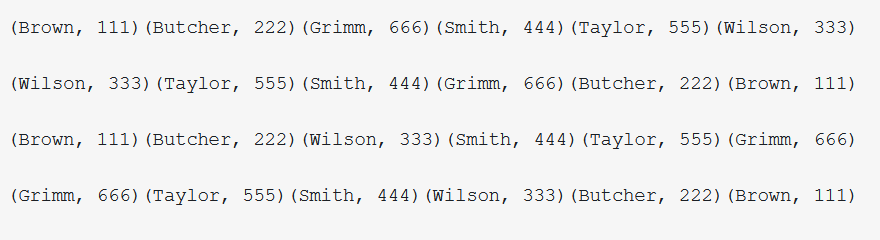
\includegraphics[width=1.0\textwidth]{content/3/chapter5/images/1-1.png}\\
\end{center}

大多数范围算法都支持投影。

\hspace*{\fill} \\ %插入空行
\noindent
\textbf{5.1.2.2\hspace{0.2cm}键和值的视图}

此外,还可以在std::unordered\_map的键(第16行)和值(第24行)上创建视图。

\begin{lstlisting}[style=styleCXX]
// rangesEntireContainer.cpp

#include <iostream>
#include <ranges>
#include <string>
#include <unordered_map>

int main() {

std::unordered_map<std::string, int> freqWord{ {"witch", 25}, {"wizard", 33},
												{"tale", 45}, {"dog", 4},
												{"cat", 34}, {"fish", 23} };

	std::cout << "Keys:" << '\n';
	auto names = std::views::keys(freqWord);
	for (const auto& name : names){ std::cout << name << " "; }
	std::cout << '\n';
	for (const auto& name : std::views::keys(freqWord)){ std::cout << name << " "; }
	
	std::cout << "\n\n";

	std::cout << "Values: " << '\n';
	auto values = std::views::values(freqWord);
	for (const auto& value : values){ std::cout << value << " "; }
	std::cout << '\n';
	for (const auto& value : std::views::values(freqWord)) {
		std::cout << value << " ";
	}

}
\end{lstlisting}

当然,键和值可以直接显示(第19和27行),输出是相同的。

\begin{tcblisting}{commandshell={}}
Keys:
fish cat dog tale wizard witch
fish cat dog tale wizard witch

Values:
23 34 4 45 33 25
23 34 4 45 33 25
\end{tcblisting}

直接在容器上工作可能没什么新奇,但支持函数组合和惰性计算会让人眼前一亮。

\subsubsubsection{5.1.3\hspace{0.2cm}函数组合}

rangesComposition.cpp中,使用的是std::map,所以键的顺序至关重要。

\begin{lstlisting}[style=styleCXX]
// rangesComposition.cpp

#include <iostream>
#include <ranges>
#include <string>
#include <map>

int main() {
	
	std::map<std::string, int> freqWord{ {"witch", 25}, {"wizard", 33},
										{"tale", 45}, {"dog", 4},
										{"cat", 34}, {"fish", 23} };
	
	std::cout << "All words: ";
	for (const auto& name : std::views::keys(freqWord)) { std::cout << name << " "; }
	
	std::cout << '\n';
	
	std::cout << "All words, reverses: ";
	for (const auto& name : std::views::keys(freqWord)
	                      | std::views::reverse) { std::cout << name << " "; }
	
	std::cout << '\n';
	
	std::cout << "The first 4 words: ";
	for (const auto& name : std::views::keys(freqWord)
	                      | std::views::take(4)) { std::cout << name << " "; }
	
	std::cout << '\n';
	
	std::cout << "All words starting with w: ";
	auto firstw = [](const std::string& name){ return name[0] == 'w'; };
	for (const auto& name : std::views::keys(freqWord)
	                      | std::views::filter(firstw)) { std::cout << name << " "; }
	
	std::cout << '\n';

}
\end{lstlisting}

这里只对键感兴趣,所以这里显示了所有的键(第15行)、反向的键(第20行)、前四行(第26行),以及以字母“w”开头的键(第32行)。

下面是程序的输出。

\begin{tcblisting}{commandshell={}}
All words: cat dog fish tale witch wizard
All words, reversed: wizard witch tale fish dog cat
The first 4 words: cat dog fish tale
All words starting with w: witch wizard
\end{tcblisting}

管道符号|属于\href{https://en.wikipedia.org/wiki/Syntactic_sugar}{语法糖},用于组合函数。组合的方式不仅可以是C(R),也可以是R | C。因此,下面的三行代码等效。

\hspace*{\fill} \\ %插入空行
\noindent
\textbf{函数组合的三种句法形式}
\begin{lstlisting}[style=styleCXX]
auto rev1 = std::views::reverse(std::views::keys(freqWord));
auto rev2 = std::views::keys(freqWord) | std::views::reverse;
auto rev3 = freqWord | std::views::keys | std::views::reverse;
\end{lstlisting}

\subsubsubsection{5.1.4\hspace{0.2cm}惰性计算}

std::views::iota是一个范围工厂,通过连续递增一个初始值来创建一个元素序列。这个序列可以有限,也可以无限。rangesIota.cpp用10个int填充std::vector,从0开始。

\begin{lstlisting}[style=styleCXX]
// rangesIota.cpp

#include <iostream>
#include <numeric>
#include <ranges>
#include <vector>

int main() {
	
	std::cout << std::boolalpha;
	
	std::vector<int> vec;
	std::vector<int> vec2;
	
	for (int i: std::views::iota(0, 10)) vec.push_back(i);
	
	for (int i: std::views::iota(0) | std::views::take(10)) vec2.push_back(i);
	
	std::cout << "vec == vec2: " << (vec == vec2) << '\n';
	
	for (int i: vec) std::cout << i << " ";

}
\end{lstlisting}

第一个iota调用(第15行)创建从0到9的所有数字,加1,第二个iota调用(第17行)创建一个无限数据流,从0开始,加1。std::views::iota(0)是惰性的。只有当请求时,才会得到一个新值。我请求了十次,所以两个vector相同。

\begin{tcblisting}{commandshell={}}
vec == vec2: true
0 1 2 3 4 5 6 7 8 9
\end{tcblisting}

现在,我想来个小挑战:找出以1,000,000以内,前20个质数。

\begin{lstlisting}[style=styleCXX]
// rangesLazy.cpp

#include <iostream>
#include <ranges>

bool isPrime(int i) {
	for (int j=2; j*j <= i; ++j){
		if (i % j == 0) return false;
	}
	return true;
}

int main() {
	
	std::cout << "Numbers from 1'000'000 to 1'001'000 (displayed each 100th): "
	          << '\n';
	for (int i: std::views::iota(1'000'000, 1'001'000)) {
		if (i % 100 == 0) std::cout << i << " ";
	}
	
	std::cout << "\n\n";
	
	auto odd = [](int i){ return i % 2 == 1; };
	std::cout << "Odd numbers from 1'000'000 to 1'001'000 (displayed each 100th): "
	          << '\n';
	for (int i: std::views::iota(1'000'000, 1'001'000) | std::views::filter(odd)) {
		if (i % 100 == 1) std::cout << i << " ";
	}
	
	std::cout << "\n\n";
	std::cout << "Prime numbers from 1'000'000 to 1'001'000: " << '\n';
	for (int i: std::views::iota(1'000'000, 1'001'000) | std::views::filter(odd)
	                                                   | std::views::filter(isPrime)) {
		std::cout << i << " ";
	}
	
	std::cout << "\n\n";
	
	std::cout << "20 prime numbers starting with 1'000'000: " << '\n';
	for (int i: std::views::iota(1'000'000) | std::views::filter(odd)
	                                        | std::views::filter(isPrime)
	                                        | std::views::take(20)) {
		std::cout << i << " ";
	}
	
	std::cout << '\n';

}
\end{lstlisting}

这是我的迭代策略:

\begin{itemize}
\item 
第18行:我不知道什么时候有20个大于1000000的质数。安全起见,我创建了1000个数字。为了方便观察,每次只展示100个。

\item 
第27行:我只对奇数感兴趣,所以去掉偶数。

\item 
第34行:现在,是时候使用下一个filter了,谓词isPrime(第7行)返回一个数字是否为素数。正如下面的截图所示,获得了75个质数。

\item 
第42行:\textit{懒惰是一种美德}。我使用std::iota作为无限大的数字工厂,从1000000开始,精确地要求20个质数。
\end{itemize}

\begin{center}
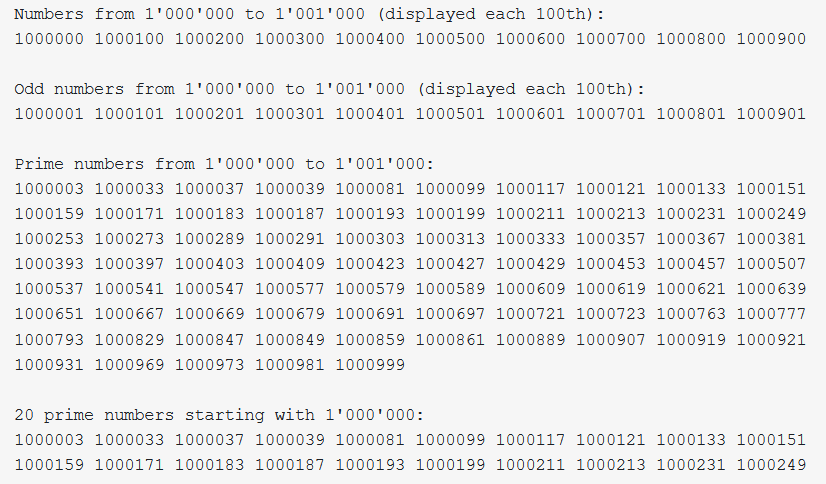
\includegraphics[width=1.0\textwidth]{content/3/chapter5/images/1-2.png}\\
找出以1,000,000以内,前20个质数
\end{center}

\subsubsubsection{5.1.5\hspace{0.2cm}自定义视图}

\hspace*{\fill} \\ %插入空行
\noindent
\textbf{5.1.5.1\hspace{0.2cm} std::ranges::view\_interface}

有了\href{https://en.cppreference.com/w/cpp/ranges/view_interface}{std::ranges::view\_interface}辅助类,可以更容易对视图进行定义。为了实现视图,自定义视图至少需要一个默认构造函数,以及成员函数begin()和end():

\begin{lstlisting}[style=styleCXX]
class MyView : public std::ranges::view_interface<MyView> {
public:
	auto begin() const { /*...*/ }
	auto end() const { /*...*/ }
};
\end{lstlisting}

通过从辅助类std::ranges::view\_interface中public派生的MyView ,并将其作为模板参数,MyView变成了一个视图。这种将类模板本身作为模板参数的技术称为\href{https://www.modernescpp.com/index.php/c-is-still-lazy}{奇异的循环模板模式}(简称CRTP)。

下一个示例中,我将使用这种技术和标准模板库的容器创建视图。

\hspace*{\fill} \\ %插入空行
\noindent
\textbf{5.1.5.2\hspace{0.2cm}容器视图}

视图ContainerView可以在任意容器上创建视图。

\begin{lstlisting}[style=styleCXX]
// containerView.cpp

#include <iostream>
#include <ranges>
#include <string>
#include <vector>

template<std::ranges::input_range Range>
requires std::ranges::view<Range>
class ContainerView : public std::ranges::view_interface<ContainerView<Range>> {
private:
	Range range_{};
	std::ranges::iterator_t<Range> begin_{ std::begin(range_) };
	std::ranges::iterator_t<Range> end_{ std::end(range_) };

public:
	ContainerView() = default;
	
	constexpr ContainerView(Range r): range_(std::move(r)) ,
									begin_(std::begin(r)), end_(std::end(r)) {}
	
	constexpr auto begin() const {
		return begin_;
	}
	constexpr auto end() const {
		return end_;
	}
};

template<typename Range>
ContainerView(Range&& range) -> ContainerView<std::ranges::views::all_t<Range>>;

int main() {

	std::vector<int> myVec{ 1, 2, 3, 4, 5, 6, 7, 8, 9};
	
	auto myContainerView = ContainerView(myVec);
	for (auto c : myContainerView) std::cout << c << " ";
	
	std::cout << '\n';
	
	for (auto i : std::views::reverse(ContainerView(myVec))) std::cout << i << ' ';
	std::cout << '\n';
	
	for (auto i : ContainerView(myVec) | std::views::reverse) std::cout << i << ' ';
	std::cout << '\n';
	
	std::cout << std::endl;
	
	std::string myStr = "Only for testing purpose.";
	
	auto myContainerView2 = ContainerView(myStr);
	for (auto c: myContainerView2) std::cout << c << " ";
	std::cout << '\n';
	
	for (auto i : std::views::reverse(ContainerView(myStr))) std::cout << i << ' ';
	std::cout << '\n';
	
	for (auto i : ContainerView(myStr) | std::views::reverse) std::cout << i << ' ';
	std::cout << '\n';

}
\end{lstlisting}

类模板ContainerView(第8行)派生自辅助类std::ranges::view\_interface,并且要求容器支持std::ranges::view(第9行)。剩下的最小的实现很简单,ContainerView有一个默认构造函数(第17行),两个必需的成员函数begin()(第22行)和end()(第25行)。方便起见,我添加了一个用户定义的类模板参数推断指南(第31行)。

main函数中,我将在std::vector(第37行)和std::string(第49行)上使用ContainerView,并向前和向后遍历它们。

\begin{center}
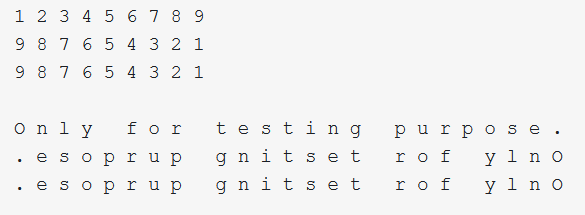
\includegraphics[width=0.6\textwidth]{content/3/chapter5/images/1-3.png}\\
\end{center}

这里提到了“类模板参数推断指南”,对于这个概念容我多说几句。

\begin{tcolorbox}[breakable,enhanced jigsaw,colback=blue!5!white,colframe=blue!75!black,title={类模板参数推断指南}]
	
C++17开始,编译器可以从模板实参推导出模板形参。模板推导指南是编译器用于推导模板参数的模式。

当使用ContainerView(myVec)时,编译器应用以下用户定义的推导指南:

\hspace*{\fill} \\ %插入空行
\noindent
\textbf{ContainerView中用户自定义的推导指南}
\begin{lstlisting}[style=styleCXX]
template<class Range>
ContainerView(Range&& range) -> ContainerView<std::ranges::views::all_t<Range>>;
\end{lstlisting}

本质上,使用Container(myVec)会导致编译器实例化箭头\texttt{->}右侧的代码:

\hspace*{\fill} \\ %插入空行
\noindent
应用容器推导指南(myVec)
\begin{lstlisting}[style=styleCXX]
ContainerView<std::ranges::views::all_t<std::vector<int>&>>(myVec);
\end{lstlisting}

\href{https://en.cppreference.com/w/cpp/language/class_template_argument_deduction}{cppreference.com}提供了类模板的用户定义推导指南的更多信息。
\end{tcolorbox}

关于范围库的下一节中,我想进行一个小实验。可以在C++中加入Python吗?

\subsubsubsection{5.1.6\hspace{0.2cm}Python的味道}

编程语言\href{https://www.python.org/}{Python}具有方便的过滤器和映射函数。

\begin{itemize}
\item 
过滤器(filter):对可迭代对象的所有元素应用谓词,并返回谓词返回true的那些元素

\item 
映射(map):对可迭代对象的所有元素使用一个函数,并返回一个包含转换后元素的新可迭代对象
\end{itemize}

C++中的可迭代对象,也可以在基于范围的for循环中使用。

此外,Python允许列表解析中组合这两个函数。

\begin{itemize}
\item 
列表解析:将过滤器和映射应用于可迭代对象,并返回一个新的可迭代对象
\end{itemize}

这就是我的挑战:尝试在C++20中使用范围库实,现类似Python的函数过滤器、映射,以及列表解析。

\hspace*{\fill} \\ %插入空行
\noindent
\textbf{5.1.6.1\hspace{0.2cm}filter}

Python的filter可以直接映射到相应的范围函数。

\hspace*{\fill} \\ %插入空行
\noindent
\textbf{C++中的filter}
\begin{lstlisting}[style=styleCXX]
/ filterRanges.cpp

#include <iostream>
#include <numeric>
#include <ranges>
#include <string>
#include <vector>

template <typename Func, typename Seq>
auto filter(Func func, const Seq& seq) {

	typedef typename Seq::value_type value_type;
	
	std::vector<value_type> result{};
	for (auto i : seq | std::views::filter(func)) result.push_back(i);
	
	return result;
}


int main() {
	
	std::cout << '\n';
	
	std::vector<int> myInts(50);
	std::iota(myInts.begin(), myInts.end(), 1);
	auto res = filter([](int i){ return (i % 3) == 0; }, myInts);
	for (auto v: res) std::cout << v << " ";
	
	
	std::vector<std::string> myStrings{"Only", "for", "testing", "purposes"};
	auto res2 = filter([](const std::string& s){ return std::isupper(s[0]); },
	                       myStrings);
	
	std::cout << "\n\n";
	
	for (auto word: res2) std::cout << word << '\n';
	
	std::cout << '\n';

}
\end{lstlisting}

解释程序之前,先展示输出效果。

\hspace*{\fill} \\ %插入空行
\begin{tcblisting}{commandshell={}}
3 6 9 12 15 18 21 24 27 30 33 36 39 42 45 48

Only
\end{tcblisting}

filter(第9行)的可读性还不错,第12行检测底层元素的类型。我只是将func应用到序列的每个元素,并返回std::vector中的元素。第27行选择从1到50的所有数字i,i需要满足条件(i \% 3) == 0。只有以大写字母开头的字符串,才能通过第32行中的过滤器。

\hspace*{\fill} \\ %插入空行
\noindent
\textbf{5.1.6.2\hspace{0.2cm}map}

map对输入序列的每个元素,使用同一个可调用对象。

\hspace*{\fill} \\ %插入空行
\noindent
\textbf{C++中的map}
\begin{lstlisting}[style=styleCXX]
// mapRanges.cpp

#include <iostream>
#include <list>
#include <ranges>
#include <string>
#include <vector>
#include <utility>


template <typename Func, typename Seq>
auto map(Func func, const Seq& seq) {

	typedef typename Seq::value_type value_type;
	using return_type = decltype(func(std::declval<value_type>()));
	
	std::vector<return_type> result{};
	for (auto i :seq | std::views::transform(func)) result.push_back(i);
	
	return result;
}

int main() {

	std::cout << '\n';
	
	std::list<int> myInts{1, 2, 3, 4, 5, 6, 7, 8, 9, 10};
	auto res = map([](int i){ return i * i; }, myInts);
	
	for (auto v: res) std::cout << v << " ";
	
	std::cout << "\n\n";
	
	std::vector<std::string> myStrings{"Only", "for", "testing", "purposes"};
	auto res2 = map([](const std::string& s){ return std::make_pair(s.size(), s); },
	                                                                myStrings);
	
	for (auto p: res2) std::cout << "(" << p.first << ", " << p.second << ") " ;
	
	std::cout << "\n\n";

}
\end{lstlisting}

map函数定义中的第15行非常有趣。表达式decltype(func(std::declval<value\_type>()))推导出return\_type。若函数func应用于输入序列的所有元素,则输入类型将转换为return\_type。std::declval<value\_type>()返回一个右值引用,decltype可以使用它来推断类型。使用map([](int i)\{return i * i;\}, myInts)(第28行)将myInt的每个元素映射为其平方值,并且使用map([](const std::string\& s)\{return std::make\_pair(s.s .size(), s);\}, myStrings)将myStrings中的每个字符串映射为pair,每个pair的第一个元素是字符串的长度。

\begin{tcblisting}{ commandshell={}}
1 4 9 16 25 36 49 64 81 100

(4, Only) (3, for) (7, testing) (8, purposes)
\end{tcblisting}

\hspace*{\fill} \\ %插入空行
\noindent
\textbf{5.1.6.3\hspace{0.2cm}列表解析}

listComprehensionRanges.cpp是对Python列表解析算法实现的简化版本。

map对输入序列的每个元素使用同一个可调用对象。

\begin{lstlisting}[style=styleCXX]
// listComprehensionRanges.cpp

#include <algorithm>
#include <cctype>
#include <functional>
#include <iostream>
#include <ranges>
#include <string>
#include <vector>
#include <utility>

template <typename T>
struct AlwaysTrue {
	constexpr bool operator()(const T&) const {
		return true;
	}
};

template <typename Map, typename Seq, typename Filt = AlwaysTrue<
                                                      typename Seq::value_type>>
auto mapFilter(Map map, Seq seq, Filt filt = Filt()) {

	typedef typename Seq::value_type value_type;
	using return_type = decltype(map(std::declval<value_type>()));
	
	std::vector<return_type> result{};
	for (auto i :seq | std::views::filter(filt)
	                 | std::views::transform(map)) result.push_back(i);
	return result;
}

int main() {

	std::cout << '\n';
	
	std::vector myInts{1, 2, 3, 4, 5, 6, 7, 8, 9, 10};
	
	auto res = mapFilter([](int i){ return i * i; }, myInts);
	for (auto v: res) std::cout << v << " ";
	
	std::cout << "\n\n";
	
	res = mapFilter([](int i){ return i * i; }, myInts,
	[](auto i){ return i % 2 == 1; });
	for (auto v: res) std::cout << v << " ";
	
	std::cout << "\n\n";
	
	std::vector<std::string> myStrings{"Only", "for", "testing", "purposes"};
	auto res2 = mapFilter([](const std::string& s){
	                          return std::make_pair(s.size(), s);
	                       }, myStrings);
	for (auto p: res2) std::cout << "(" << p.first << ", " << p.second << ") " ;
	
	std::cout << "\n\n";
	
	myStrings = {"Only", "for", "testing", "purposes"};
	res2 = mapFilter([](const std::string& s){
	                     return std::make_pair(s.size(), s);
	                 }, myStrings,
	                [](const std::string& word){ return std::isupper(word[0]); });
	
	for (auto p: res2) std::cout << "(" << p.first << ", " << p.second << ") " ;
	
	std::cout << "\n\n";

}
\end{lstlisting}

过滤器函数使用的默认谓词(第19行)总返回true(第12行),所以mapFilter函数在默认情况下只是作为一个映射函数,所以mapFilter函数在第38行和第50行中的行为与前面的map函数相同。第42和55行在一次调用中同时应用map和filter函数。

\begin{tcblisting}{commandshell={}}
1 4 9 16 25 36 49 64 81 100

1 9 25 49 81

(4, Only) (3, for) (7, testing) (8, purposes)

(4, Only)
\end{tcblisting}

\begin{tcolorbox}[breakable,enhanced jigsaw,colback=mygreen!5!white,colframe=mygreen!75!black,title={总结}]
\begin{itemize}
\item 
范围库为我们提供了STL算法的特殊版本。范围库算法是惰性的,可以直接工作在容器上,并且可以组合。

\item 
范围库的算法
\begin{itemize}
\item 
惰性,因此可以在无限的数据流上调用。

\item 
可以直接操作容器,不需要由两个迭代器定义的范围。

\item 
可以使用管道(|)符号进行组合。
\end{itemize}
\end{itemize}
\end{tcolorbox}	
	
\newpage
	
	
	
	
	
	
	
	
	
	
	
	
	
	
	
	
	
	
	
	
	